%%%%%%%%%%%%%%%%%%%%%%%%%%%%%%%%%%%%%%%%%%%%%%%%%%%%%%%%%%%%%%%%%%%%
%
%   Style for CMS Computing / Physics Technical Design Reports
%
%   Lucas Taylor  4 Feb 2005,   Revised  12 Oct 2005
%
%%%%%%%%%%%%%%%%%%%%%%%%%%%%%%%%%%%%%%%%%%%%%%%%%%%%%%%%%%%%%%%%%%%%

%  the following line is edited by the tdr script to change or to pass
%  additional options:
\documentclass[11pt,twoside,a4paper,pdftex,cmspaper]{cms-tdr}

%%%%%%%%%%%%%%%%%%%%%%%%%%%%%%%%%%%%%%%%%%%%%%%%%%%%%%%%%%%%%%%%%%%%

\begin{document}\cmsNoteHeader{CFT-09-016}
%%%%%%%%%%%%%%%%%%%%%%%%%%%%%%%%%%%%%%%%%%%%%%%%%%%%%%%%%%%%%%%%%%%%
%
%  Common definitions
%
%  N.B. use of \providecommand rather than \newcommand means
%       that a definition is ignored if already specified
%
%                                              L. Taylor 18 Feb 2005
%%%%%%%%%%%%%%%%%%%%%%%%%%%%%%%%%%%%%%%%%%%%%%%%%%%%%%%%%%%%%%%%%%%%


%%%%%%%%%%%%%%%%%%%%%%%%%%%%%%%%%%%%%%%%%%%%%%%%%%%%%%%%%%%%%%%%%%%%
%
% Hyphenations (only need to add here if you get a nasty word break)
%
\hyphenation{env-iron-men-tal}%    just an example
\hyphenation{had-ron-i-za-tion}
\hyphenation{cal-or-i-me-ter}
\hyphenation{de-vices}
%
% Hyphenations-end
%% CVS info. These are modified by cvs at checkout time.
% The last version of these macros found before the maketitle will be the one on the front page,
% so only the main file is tracked.
% Edit by hand with care!
\RCS$Revision: 1.11 $
\RCS$Date: 2009/07/22 19:24:35 $
\RCS$Name:  $
%%%%%%%%%%%%% ptdr definitions %%%%%%%%%%%%%%%%%%%%%
\input{ptdr-definitions}
%%%%%%%%%%%%%%%  Title page %%%%%%%%%%%%%%%%%%%%%%%%
\cmsNoteHeader{09-016}
\title{Alignment of the CMS Muon System with \\ Cosmic Ray and Beam-Halo Tracks}% Force line breaks with \\

%Author is always "The CMS Collaboration" for PAS, so author, etc will be ignored
\address[cern]{CERN}
\address[su]{Some University}
\author[su]{Some Cool Dudes}\author[cern]{A. Cern Person}

% please supply the date in yyyy/mm/dd format. Today has been
% redefined to do so, but it should be fixed as of the final release date.
\date{\today}

% note that you cannot use \verb in the abstract text
\abstract{
\input{abstract}
}

% these need to be filled in by hand and should (MUST) match the info
% in the TeX equivalents less the TeX markup
\hypersetup{%
pdfauthor={Some Cool Dudes, A. Cern Person},%
pdftitle={Muon Track-based alignment},%
pdfsubject={CMS},%
pdfkeywords={CMS, detectors, alignment, tracks}}

\maketitle %maketitle comes after all the front information has been supplied

%%%%%%%%%%%%%%%%%%%%%%%%%%%%%%%%  Begin text %%%%%%%%%%%%%%%%%%%%%%%%%%%%%
\tableofcontents

%---------------------------------------------------------------------
\section{Introduction and Geometry}
\input{intro_geom}

%---------------------------------------------------------------------
\section{Local DT Alignment}
\label{sec:localdt}
\input{standalone_dt_alignment}

%---------------------------------------------------------------------
\section{Local CSC Alignment}
\label{sec:localcsc}
\input{csc_overlaps_alignment}

%---------------------------------------------------------------------
\section{Global Muon Alignment}
\label{sec:global_muon_alignment}

Local muon alignment procedures arrange sets of chambers in
self-consistent coordinate systems, but cannot relate those
coordinates to the locations of other subsystems of CMS, particularly
the tracker.  In this section, we describe methods to
align muon chambers relative to the tracker, such that all
tracking volumes in CMS share one global system of coordinates.  Since
these global alignment methods are partly independent of the local alignments,
they can be used to cross-check each other.

Two algorithms, HIP (Hits and Impact Points) and Millepede, have been
developed to align muon chambers relative to the tracker.  Each is
described in its own section below, followed by studies in Monte Carlo
simulations, and then results of each with cosmic ray data.

\subsection{The HIP Algorithm}
\label{sec:hipalgo}
\input{gma_hip_algorithm}  

\subsection{The MilliPede Algorithm}
\input{gma_mp_algorithm}  

\subsection{Monte Carlo Study and Discussion of Systematic Errors}
\input{mc_and_syst_studies}

\subsection{Global Alignment Results and Cross-Checks}
Both the HIP and Millepede algorithms were applied to align a subset
of barrel chambers during the CRAFT
data-taking run.  Wheels $-$1, 0, and $+$1 were aligned, with the
exception of sectors 1 and 7 (extreme horizontal sides of the
detector) using the barrel section of the tracker as the track
reference.  The alignment was restricted to this central subset of the
barrel chambers because they were the only ones sufficiently
illuminated by the primarily vertical distribution of cosmic rays.  We
also restricted the input to high-quality $100 < p_T < 200$~GeV tracks
with at least 15 tracker hits and a tracker reduced $\chi^2 < 10$.
Loosening these cuts does not make significantly more chambers
available for alignment.  The dataset included all runs marked as acceptable for
physics in the CMS run registry, with a magnetic field of 3.8~T.  The
CRAFT period included several on-off cycles of the magnetic field,
which were shown to result in reproducible alignments with the
hardware system~\cite{ref:hardware_alignment} and tracks (within
statistical precision).

In addition to the chambers explicitly excluded from alignment due to
poor statistics, two chambers next to sectors 1 and 7 (in wheel,
station, sector ($-$1, 2, 8) and ($+$1, 3, 8)) had no tracks passing
the cuts and two more (($-$1, 1, 12) and ($+$1, 2, 2)) failed to
converge in HIP, owing to the extreme azimuthal asymmetry of cosmic
rays underground.

We checked our alignment results in four ways: we verified (1) that
the algorithms optimized their intended expressions, (2) that they
agree with one another, (3) that the new global chamber positions yield the same or
better agreement with local measurements, and (4) that the new
alignment yields better momentum resolution for tracks.

The simplest way to test the internal consistency of the algorithm (1)
is to run the alignment algorithm a second time on the same dataset
and verify that the second alignment corrections are always zero.  As
a sanity check, we also verified that the raw residuals distributions
are centered at zero with very high precision.  An example of this was
shown in Figure~\ref{fig:examplefit}.

To demonstrate that the two algorithms agree with each other (2), we
present corrections computed by each algorithm in a scatter
plot~\ref{fig:sidebyside}.  Though the corrections were on the order
of 0.5--3~mm/mrad, the two algorithms agree with each other within
expectations from the Monte Carlo study (Figure~\ref{fig:hip_MC}).  The
two parameters in which no correlation is observed between the
algorithms are $\delta_z$ and $\delta_{\phi_z}$, which are the most
likely to be affected by the treatment of tails in residuals
distributions.  The distributions of $\delta_y$ and $\delta_{\phi_x}$
have tall peaks at zero: these parameters cannot be aligned in
station~4, because station~4 chambers do not measure $\Delta y$
residuals.

\begin{figure}
\begin{center}
%% \includegraphics[width=0.32\linewidth]{plots/gma_hip_results/delta_xComparison.pdf}
%% \includegraphics[width=0.32\linewidth]{plots/gma_hip_results/delta_yComparison.pdf}
%% \includegraphics[width=0.32\linewidth]{plots/gma_hip_results/delta_zComparison.pdf}

%% \includegraphics[width=0.32\linewidth]{plots/gma_hip_results/phixComparison.pdf}
%% \includegraphics[width=0.32\linewidth]{plots/gma_hip_results/phiyComparison.pdf}
%% \includegraphics[width=0.32\linewidth]{plots/gma_hip_results/phizComparison.pdf}

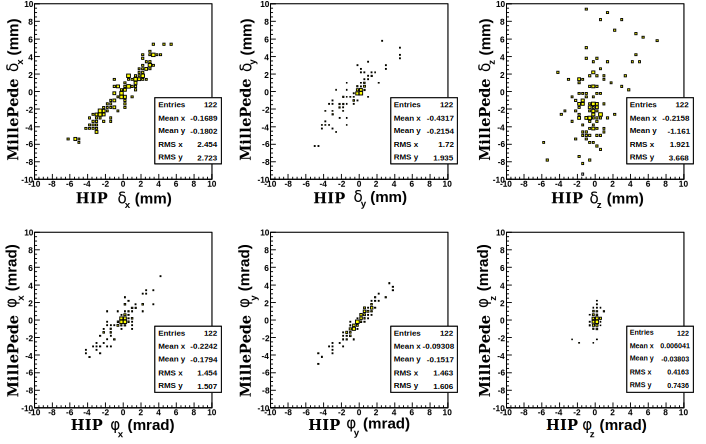
\includegraphics[width=\linewidth]{plots/gma_hip_results/MP-V4_vs_HIP-V4.pdf}
\end{center}
\caption{Alignment corrections determined by the HIP and Millepede algorithms. (Only aligned chambers are shown.)\label{fig:sidebyside}}
\end{figure}

Local alignment measurements to test consistency between global data
and local data (3) were derived by extrapolating linear track segments
from one chamber to the next (in the same sector, neighboring
stations).  This verification procedure introduces information not
used in the alignment itself, namely the higher precision with which
tracks can be propagated over a short distance (1~meter) than a long
distance (3--6~meters).

For this diagnostic, tracks were selected with $p_T > 50$~GeV and a
correction was applied to cancel the effect of the magnetic field by
taking advantage of the fact that positively- and negatively-charged
tracks are pushed in opposite directions.
%% Figure~\ref{fig:valid_DTconsts} shows the level of agreement in $x$
%% position and $\frac{dx}{dz}$ angle between segments in neighboring
%% stations for each sector in wheel~0.
To compare the initial state with the results of each algorithm in all
station-pairs, sectors, and wheels, we filled histograms with the
fitted Gaussian peak of each comparison, shown in
Figure~\ref{fig:valid_NOMvsMPvsHIP}.  Though the global algorithms
changed the positions of chambers by 2.5~mm in $\delta_x$ and 1.5~mrad
in $\delta_{\phi_y}$ (RMS in Figure~\ref{fig:sidebyside}), local
differences of 0.8--1.3~mm and 1.0--1.3~mrad are not only maintained
but reduced by 10\% to as much as a factor of 2.  As expected, the chambers which are closest
to the tracker (station~1-to-2 differences) are the most precisely
aligned.  The individual outliers in station~4 contain internal
structure in their residuals distributions which are the subject of
further study.

%% \begin{figure}
%%   \centering
%%   \subfigure[Average $x$ difference between stations]{\includegraphics[width=0.4\textwidth, angle=90]{plots/validation/aligVal_08June09_LocalX_YB0.pdf}}
%%   \subfigure[Average $\frac{dx}{dz}$ difference between stations]{\includegraphics[width=0.4\textwidth, angle=90]{plots/validation/aligVal_08June09_Phi_YB0.pdf}}
%%   \caption{Validation of DT alignment by comparing track segments in
%%   neighboring chambers (after alignment using the HIP algorithm).\label{fig:valid_DTconsts}}
%% \end{figure}
 
\begin{figure}
  \centering
  \subfigure[Before global alignment]{\includegraphics[width=0.4\textwidth, angle=90]{plots/gma_hip_results/YB0YB1YBm1_V4_38T.pdf}}
  \subfigure[Results from the HIP algorithm]{\includegraphics[width=0.45\textwidth, angle=90]{plots/validation/meanHisto_HIP_onlyAlign.pdf}}
  \subfigure[Results from the Millepede algorithm]{\includegraphics[width=0.45\textwidth, angle=90]{plots/validation/meanHisto_Millepede.pdf}}
  \caption{Local differences in alignment as measured by segments.  Each histogram entry is a pair of chambers in neighboring stations, but the same wheel and sector.  The three histograms show station~1-to-2 differences (blue), 2-to-3 differences (red), and 3-to-4 differences (green).  \label{fig:valid_NOMvsMPvsHIP}}
\end{figure}
 
To verify that the new alignment (in this case, HIP only) improves
momentum resolution (4), we selected cosmic rays with $p_T > 200$~GeV,
split each into two tracks near the origin (similar to what would be
observed in LHC collisions), and compared the momentum of the top and
bottom fits.  Since the cosmic ray muon is a single particle, any
mismatch between the halves is purely instrumental.  Cosmic rays have
a steeply falling distribution, so most of the selected tracks have
$p_T$ close to 200~GeV.  The alignment was performed using tracks with
$100 < p_T < 200$~GeV tracks, so the diagnostic sample is
statistically independent from the alignment.
Figure~\ref{fig:chargesplitting} compares tracker-only tracks and
tracks reconstructed with muon hits (first muon station only), before
and after the global muon alignment.

\begin{figure}
  \centering
  \subfigure[Before global muon alignment]{\includegraphics[width=0.45\linewidth]{plots/monitoring_validation/chargesplitting_withoutalignment.pdf}}
  \subfigure[Results from the HIP algorithm]{\includegraphics[width=0.45\linewidth]{plots/monitoring_validation/chargesplitting_withalignment.pdf}}
  \caption{Top vs.~bottom $1/p_T$ comparison for $p_T \gtrsim 200$~GeV split cosmic rays.\label{fig:chargesplitting}}
\end{figure}
  

%---------------------------------------------------------------------
\section{Conclusions}
In this note, we have demonstrated a variety of software procedures for
aligning different parts of the muon system: layers in DT chambers,
CSC chambers in rings, and global positions of DT chambers relative to
the central tracker, using charged tracks.  We have fully exploited the available data,
horizontal LHC beam-halo muons and vertical cosmic rays.

These procedures will be used without major modifications to re-align
the muon system with muons from LHC collisions, once such data are
available.  The azimuthally-symmetric and broad pseudorapidity
distribution of collisions muons will allow us to extend the global
alignment to all muon chambers.  Although the endcap chambers are
sensitive to only three parameters, $\delta_{r\phi}$,
$\delta_{\phi_y}$ and $\delta_{\phi_z}$ (the same as local CSC
alignment), these parameters can be determined with 400~$\mu$m,
0.4~mrad, and 0.6~mrad resolution with similar results for all degrees
of freedom in the muon barrel, according to 50~pb$^{-1}$ simulations.
To constrain the remaining CSC parameters, we can exploit the
complementarity of the endcap hardware alignment
system~\cite{ref:hardware_alignment} (which measure $\delta_z$ and
$\delta_{\phi_x}$ directly), and independently test its validity in
$\delta_{r\phi}$.

Moreover, the addition of collisions muons and larger beam-halo
datasets will allow new cross-checks to be performed, as the local CSC
alignment (section~\ref{sec:localcsc}) and CSC layer alignment can be
performed with both collisions and beam-halo, so we can doubly
cross-check by performing the same method with different track sources
and different methods with the same track source.  Similarly,
collisions and cosmic rays can both be used in the barrel, and they
differ in how the reference tracks sample the tracker, and hence
potental input track bias.

By verifying the muon alignment in as many ways as possible, we can
add confidence to the muon momentum resolution at all energy scales,
improving sensitivity to signatures of new physics.


%---------------------------------------------------------------------
\bibliography{auto_generated}   % will be created by the tdr script.

\end{document}

